\documentclass[12pt]{article}

\usepackage{amsmath}
\usepackage{array}
\usepackage{caption}
\usepackage[top=1in, bottom=1in, left=0.75in, right=0.75in]{geometry}
\usepackage{graphicx}
\usepackage[colorlinks=true, allcolors=blue]{hyperref}
\usepackage[utf8]{inputenc}
\usepackage{multirow}
\usepackage{pdfpages}
\usepackage[section]{placeins}

\graphicspath{{./figures/}}

\title{ECE 271: Chapter 3 Reading Report}
\author{Phi Luu}
\date{October 15\textsuperscript{th}, 2018}

\begin{document}

\maketitle

%%%%%%%%%%%%%%%%%%%%%%%%%%%%%%%%%%%%%%%%%%%%%%%%%%%%%%%%%%%%%%%%%%%%%%%%%%%%%%%%
% Chapter Outline
%%%%%%%%%%%%%%%%%%%%%%%%%%%%%%%%%%%%%%%%%%%%%%%%%%%%%%%%%%%%%%%%%%%%%%%%%%%%%%%%
\section{Chapter Outline}

This chapter covers ...

%%%%%%%%%%%%%%%%%%%%%%%%%%%%%%%%%%%%%%%%
% Introduction
%%%%%%%%%%%%%%%%%%%%%%%%%%%%%%%%%%%%%%%%
\subsection{Introduction}

%%%%%%%%%%%%%%%%%%%%%%%%%%%%%%%%%%%%%%%%
% Latches and Flip-Flops
%%%%%%%%%%%%%%%%%%%%%%%%%%%%%%%%%%%%%%%%
\subsection{Latches and Flip-Flops}

[Opening paragraph, if any]

\begin{enumerate}
    %%%%%%%%%%%%%%%%%%%%
    % Latches and Flip-Flops
    %%%%%%%%%%%%%%%%%%%%
    \item \textbf{Latches and Flip-Flops}

    %%%%%%%%%%%%%%%%%%%%
    % D Latch
    %%%%%%%%%%%%%%%%%%%%
    \item \textbf{D Latch}

    %%%%%%%%%%%%%%%%%%%%
    % D Flip-Flop
    %%%%%%%%%%%%%%%%%%%%
    \item \textbf{D Flip-Flop}

    %%%%%%%%%%%%%%%%%%%%
    % Register
    %%%%%%%%%%%%%%%%%%%%
    \item \textbf{Register}

    %%%%%%%%%%%%%%%%%%%%
    % Enabled Flip-Flop
    %%%%%%%%%%%%%%%%%%%%
    \item \textbf{Enabled Flip-Flop}

    %%%%%%%%%%%%%%%%%%%%
    % Resettable Flip-Flop
    %%%%%%%%%%%%%%%%%%%%
    \item \textbf{Resettable Flip-Flop}

    %%%%%%%%%%%%%%%%%%%%
    % Transistor-Level Latch and Flip-Flop Designs
    %%%%%%%%%%%%%%%%%%%%
    \item \textbf{Transistor-Level Latch and Flip-Flop Designs}

    %%%%%%%%%%%%%%%%%%%%
    % Putting It All Together
    %%%%%%%%%%%%%%%%%%%%
    \item \textbf{Putting It All Together}
\end{enumerate}

%%%%%%%%%%%%%%%%%%%%%%%%%%%%%%%%%%%%%%%%
% Synchronous Logic Design
%%%%%%%%%%%%%%%%%%%%%%%%%%%%%%%%%%%%%%%%
\subsection{Synchronous Logic Design}

[Opening paragraph, if any]

\begin{enumerate}
    %%%%%%%%%%%%%%%%%%%%
    % Some Problematic Circuits
    %%%%%%%%%%%%%%%%%%%%
    \item \textbf{Some Problematic Circuits}

    %%%%%%%%%%%%%%%%%%%%
    % Synchronous Sequential Circuits
    %%%%%%%%%%%%%%%%%%%%
    \item \textbf{Synchronous Sequential Circuits}

    %%%%%%%%%%%%%%%%%%%%
    % Synchronous and Asynchronous Circuits
    %%%%%%%%%%%%%%%%%%%%
    \item \textbf{Synchronous and Asynchronous Circuits}
\end{enumerate}

%%%%%%%%%%%%%%%%%%%%%%%%%%%%%%%%%%%%%%%%
% Finite State Machines
%%%%%%%%%%%%%%%%%%%%%%%%%%%%%%%%%%%%%%%%
\subsection{Finite State Machines}

[Opening paragraph, if any]

\begin{enumerate}
    %%%%%%%%%%%%%%%%%%%%
    % FSM Design Examples
    %%%%%%%%%%%%%%%%%%%%
    \item \textbf{FSM Design Example}

    %%%%%%%%%%%%%%%%%%%%
    % State Encodings
    %%%%%%%%%%%%%%%%%%%%
    \item \textbf{State Encodings}

    %%%%%%%%%%%%%%%%%%%%
    % Moore and Mealy Machines
    %%%%%%%%%%%%%%%%%%%%
    \item \textbf{Moore and Mealy Machines}


    %%%%%%%%%%%%%%%%%%%%
    % Factoring State Machines
    %%%%%%%%%%%%%%%%%%%%
    \item \textbf{Factoring State Machines}

    %%%%%%%%%%%%%%%%%%%%
    % Deriving an FSM from a Schematic
    %%%%%%%%%%%%%%%%%%%%
    \item \textbf{Deriving an FSM from a Schematic}

    %%%%%%%%%%%%%%%%%%%%
    % FSM Review
    %%%%%%%%%%%%%%%%%%%%
    \item \textbf{FSM Review}
\end{enumerate}

%%%%%%%%%%%%%%%%%%%%%%%%%%%%%%%%%%%%%%%%
% Timing of Sequential Logic
%%%%%%%%%%%%%%%%%%%%%%%%%%%%%%%%%%%%%%%%
\subsection{Timing of Sequential Logic}

[Opening paragraph, if any]

\begin{enumerate}
    %%%%%%%%%%%%%%%%%%%%
    % The Dynamic Discipline
    %%%%%%%%%%%%%%%%%%%%
    \item \textbf{The Dynamic Discipline}

    %%%%%%%%%%%%%%%%%%%%
    % System Timing
    %%%%%%%%%%%%%%%%%%%%
    \item \textbf{System Timing}

    %%%%%%%%%%%%%%%%%%%%
    % Clock Skew
    %%%%%%%%%%%%%%%%%%%%
    \item \textbf{Clock Skew}

    %%%%%%%%%%%%%%%%%%%%
    % Metastability
    %%%%%%%%%%%%%%%%%%%%
    \item \textbf{Metastability}

    %%%%%%%%%%%%%%%%%%%%
    % Synchronizers
    %%%%%%%%%%%%%%%%%%%%
    \item \textbf{Synchronizers}

    %%%%%%%%%%%%%%%%%%%%
    % Derivation of Resolution Time
    %%%%%%%%%%%%%%%%%%%%
    \item \textbf{Derivation of Resolution Time}
\end{enumerate}

%%%%%%%%%%%%%%%%%%%%%%%%%%%%%%%%%%%%%%%%
% Parallelism
%%%%%%%%%%%%%%%%%%%%%%%%%%%%%%%%%%%%%%%%
\subsection{Parallelism}

%%%%%%%%%%%%%%%%%%%%%%%%%%%%%%%%%%%%%%%%
% Summary
%%%%%%%%%%%%%%%%%%%%%%%%%%%%%%%%%%%%%%%%
\subsection{Summary}

%%%%%%%%%%%%%%%%%%%%%%%%%%%%%%%%%%%%%%%%%%%%%%%%%%%%%%%%%%%%%%%%%%%%%%%%%%%%%%%%
% Grey Box Exploration
%%%%%%%%%%%%%%%%%%%%%%%%%%%%%%%%%%%%%%%%%%%%%%%%%%%%%%%%%%%%%%%%%%%%%%%%%%%%%%%%
\section{Grey Box Exploration}

\begin{enumerate}
    %%%%%%%%%%%%%%%%%%%%%%%%%%%%%%%%%%%%%%%%
    % First grey box
    %%%%%%%%%%%%%%%%%%%%%%%%%%%%%%%%%%%%%%%%
    \item The first blurb is on page ...

    %%%%%%%%%%%%%%%%%%%%%%%%%%%%%%%%%%%%%%%%
    % Second grey box
    %%%%%%%%%%%%%%%%%%%%%%%%%%%%%%%%%%%%%%%%
    \item The second blurb is on page ...
\end{enumerate}

%%%%%%%%%%%%%%%%%%%%%%%%%%%%%%%%%%%%%%%%%%%%%%%%%%%%%%%%%%%%%%%%%%%%%%%%%%%%%%%%
% Figures
%%%%%%%%%%%%%%%%%%%%%%%%%%%%%%%%%%%%%%%%%%%%%%%%%%%%%%%%%%%%%%%%%%%%%%%%%%%%%%%%
\section{Figures}

Two figures were selected from this chapter for special recognition. Figure[...] was selected ...

% \begin{figure}[h]
%     \centering
%     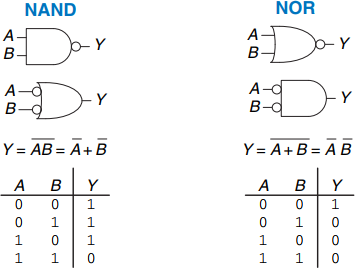
\includegraphics[width=0.5\textwidth]{de_morgan_gates.png}
%     \caption{De Morgan equivalent gates and their truth tables}
%     \label{figure:9}
% \end{figure}

Figure[...] was selected ...

% \begin{figure}[h]
%     \centering
%     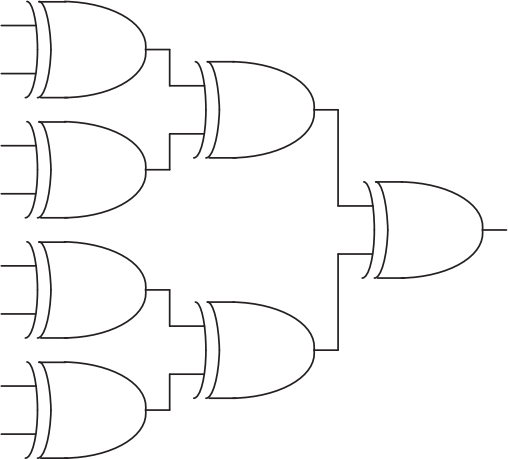
\includegraphics[width=0.25\textwidth]{eight_input_xor}
%     \caption{An eight-input XOR constructed from seven two-input XOR}
%     \label{figure:10}
% \end{figure}

%%%%%%%%%%%%%%%%%%%%%%%%%%%%%%%%%%%%%%%%%%%%%%%%%%%%%%%%%%%%%%%%%%%%%%%%%%%%%%%%
% Example Problems
%%%%%%%%%%%%%%%%%%%%%%%%%%%%%%%%%%%%%%%%%%%%%%%%%%%%%%%%%%%%%%%%%%%%%%%%%%%%%%%%
\section{Example Problems}

See the attached images on the next pages.

% 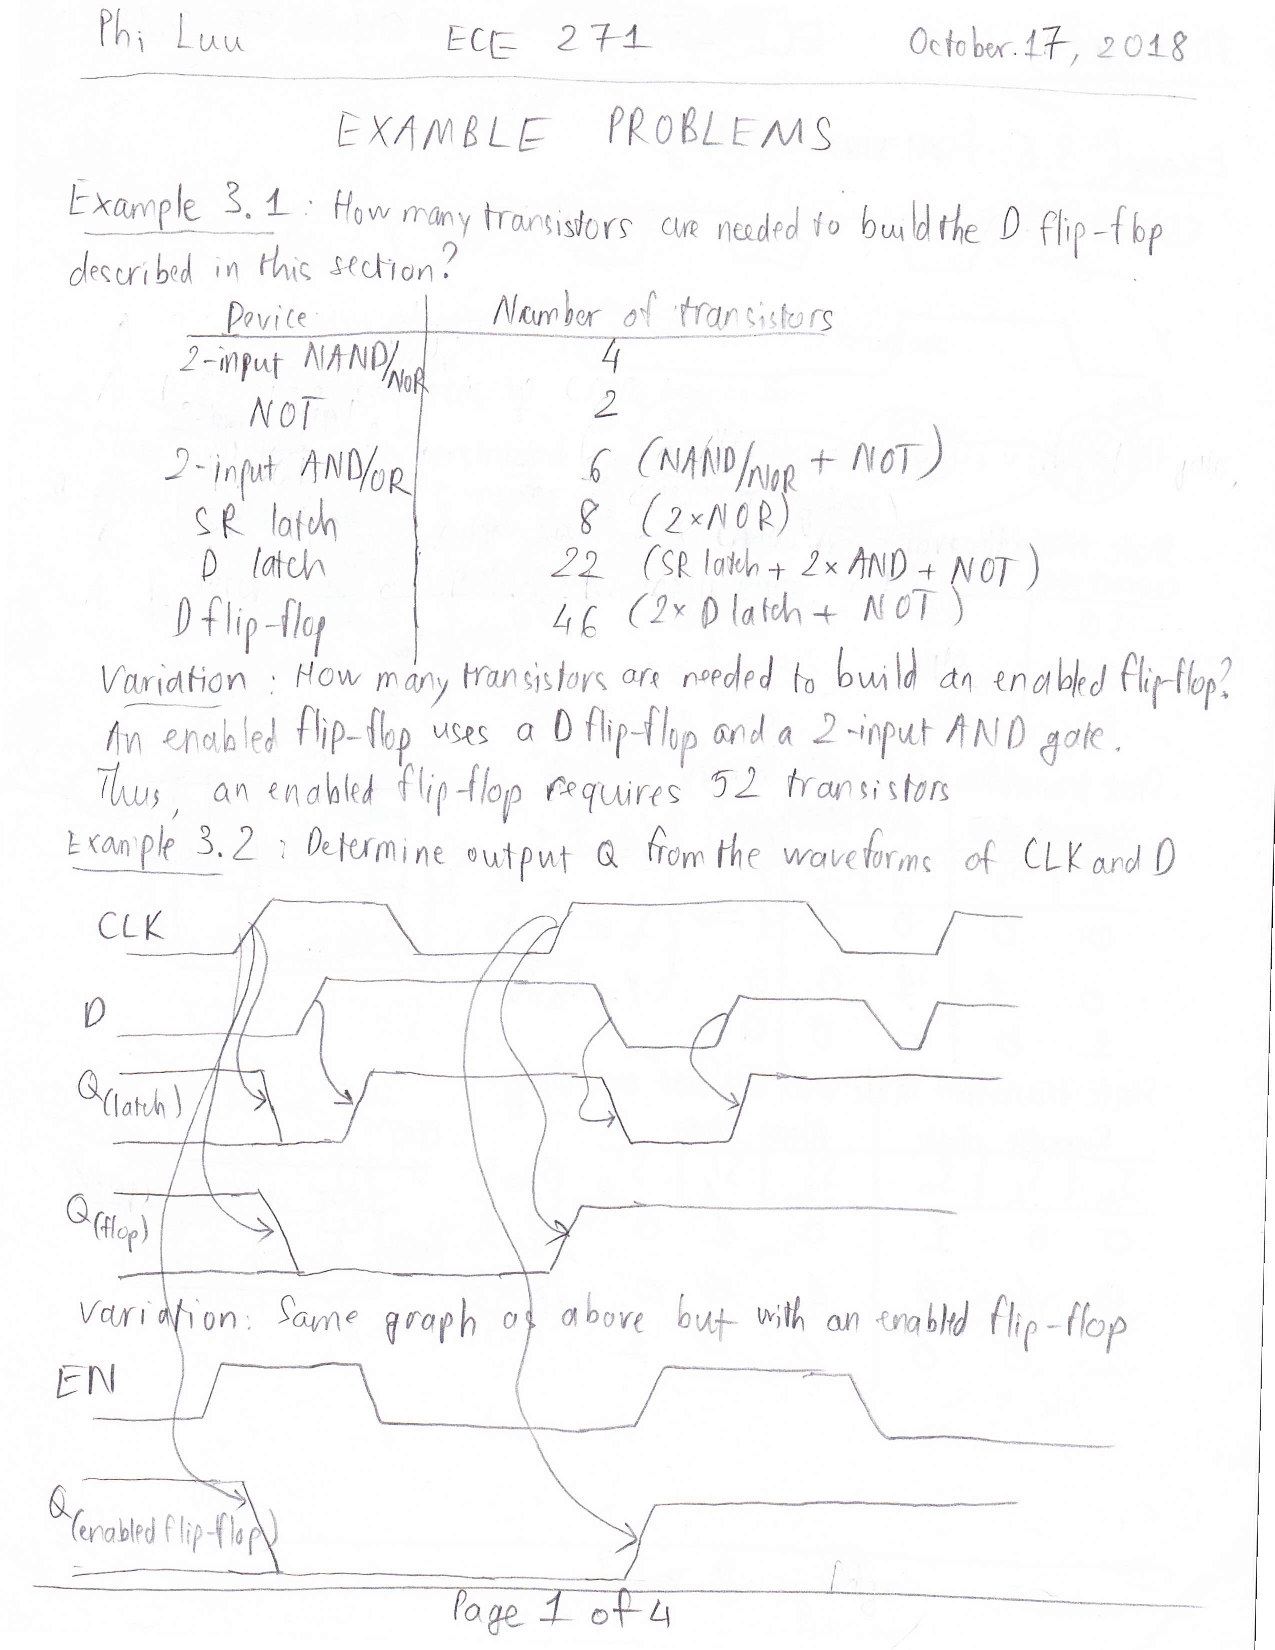
\includepdf[page=-]{example_problems}

%%%%%%%%%%%%%%%%%%%%%%%%%%%%%%%%%%%%%%%%%%%%%%%%%%%%%%%%%%%%%%%%%%%%%%%%%%%%%%%%
% Glossary
%%%%%%%%%%%%%%%%%%%%%%%%%%%%%%%%%%%%%%%%%%%%%%%%%%%%%%%%%%%%%%%%%%%%%%%%%%%%%%%%
\section{Glossary}

All definitions were found from the Google search engine, typing "define ..." for the first item.

\begin{enumerate}
    \item Circuit

    noun:

    \begin{enumerate}
        \item a roughly circular line, route, or movement that starts and finishes at the same place.
        \item an established itinerary of events or venues used for a particular activity, typically involving public performance.
    \end{enumerate}

    verb:

    \begin{enumerate}
        \item move all the way around (a place or thing).
    \end{enumerate}

    \item Boolean

    adjective:

    \begin{enumerate}
        \item denoting a system of algebraic notation used to represent logical propositions, especially in computing and electronics.
    \end{enumerate}

    noun:

    \begin{enumerate}
        \item a binary variable, having two possible values called ``true" and ``false."
    \end{enumerate}

    \item{Combination}

    noun:

    \begin{enumerate}
        \item a joining or merging of different parts or qualities in which the component elements are individually distinct.
        \item a sequence of numbers or letters used to open a combination lock.
    \end{enumerate}

    \item{Axiom}

    noun:

    \begin{enumerate}
        \item a statement or proposition that is regarded as being established, accepted, or self-evidently true.
    \end{enumerate}

    \item{Theorem}

    noun:

    \begin{enumerate}
        \item a general proposition not self-evident but proved by a chain of reasoning; a truth established by means of accepted truths.
    \end{enumerate}
\end{enumerate}

%%%%%%%%%%%%%%%%%%%%%%%%%%%%%%%%%%%%%%%%%%%%%%%%%%%%%%%%%%%%%%%%%%%%%%%%%%%%%%%%
% Interview Question
%%%%%%%%%%%%%%%%%%%%%%%%%%%%%%%%%%%%%%%%%%%%%%%%%%%%%%%%%%%%%%%%%%%%%%%%%%%%%%%%
\section{Interview Question}

See the attached image on the next page.

% 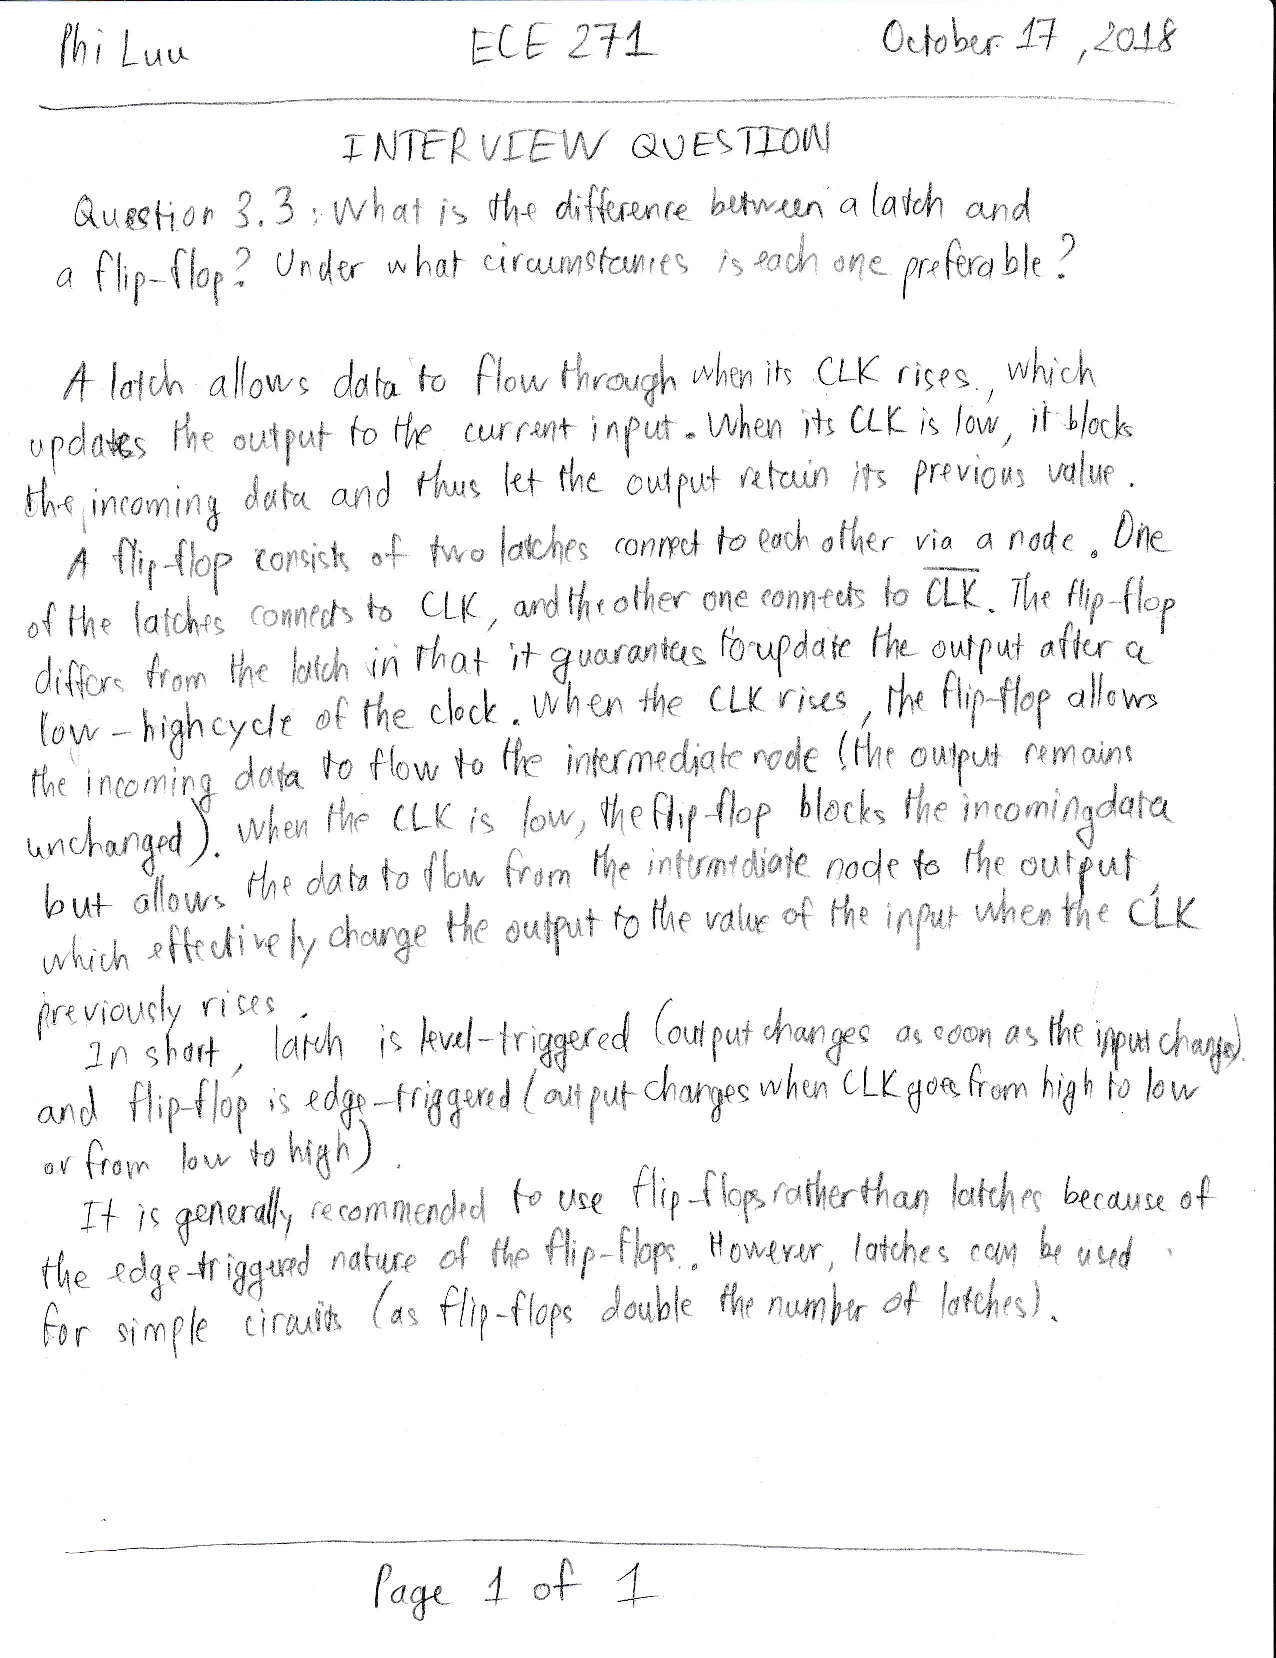
\includepdf[page=-]{interview_question}

%%%%%%%%%%%%%%%%%%%%%%%%%%%%%%%%%%%%%%%%%%%%%%%%%%%%%%%%%%%%%%%%%%%%%%%%%%%%%%%%
% Reflection
%%%%%%%%%%%%%%%%%%%%%%%%%%%%%%%%%%%%%%%%%%%%%%%%%%%%%%%%%%%%%%%%%%%%%%%%%%%%%%%%
\section{Reflection}

%%%%%%%%%%%%%%%%%%%%%%%%%%%%%%%%%%%%%%%%%%%%%%%%%%%%%%%%%%%%%%%%%%%%%%%%%%%%%%%%
% Questions for Lecture
%%%%%%%%%%%%%%%%%%%%%%%%%%%%%%%%%%%%%%%%%%%%%%%%%%%%%%%%%%%%%%%%%%%%%%%%%%%%%%%%
\section{Questions for Lecture}

\begin{enumerate}
    \item What are the applications of multiplexers? Can you show me a real-life example of a multiplexer?
    \item What determines which input will be taken into account in a tristate buffer?
    \item Electronic devices, such as smartphones, are getting smaller and faster but also more expensive. Do you favor speed or cost?
\end{enumerate}

%%%%%%%%%%%%%%%%%%%%%%%%%%%%%%%%%%%%%%%%%%%%%%%%%%%%%%%%%%%%%%%%%%%%%%%%%%%%%%%%
% Bibliography
%%%%%%%%%%%%%%%%%%%%%%%%%%%%%%%%%%%%%%%%%%%%%%%%%%%%%%%%%%%%%%%%%%%%%%%%%%%%%%%%
\bibliographystyle{ieeetr}
\bibliography{references}

\end{document}
